% !TEX root = thesis.tex

\section{Aplicacions}\label{sec:Aplicacions}

En aquesta secció veurem de forma general diferents aplicacions tant de teoria de nusos com de topologia en diferents camps de la ciència. Algunes d'aquestes aplicacions son ben conegudes i altres son relativament recents.\\

Durant molt de temps no es tenia clar si la topologia era una eina útil per descriure el comportament de partícules subatòmiques. Això es deu als efectes de la física quàntica sobre sistemes o partícules realment petites que poden ser descrits mitjançant la funció d'ona. Gràcies a les contribucions de David Thouless, Duncan Haldane i Michael Kosterlitz que van guanyar el premi nobel de física l'any 2016 van adonar-se de l'existència de propietats topològiques a l'escala quàntica. Des de llavors, aquest descobriment ha obert la porta a una revolució en la ciència de materials, enginyeria electrònica i ciència de la computació. Repassarem algunes de les aplicacions que han sorgit a conseqüència d'aquest descobriment i fem al·lusió a resultats de Alexei Kitaev i Edward Witten sobre la computació quàntica i la construcció dels primers ordinadors quàntics.

\subsection{Aïllants topològics}\label{sec:aillanttopologic}
 Per tal de motivar la Secció \ref{sec:nusosquantics} començarem discutint un fenòmen ben conegut pels físics. A \cite{topologicalinsulators} s'estudia aquest fenòmen en detall. Aquesta es tracta d'una propietat que presenten diferents materials al ser exposats a un camp magnètic.\\
 
 Si imaginem que disposem d'una làmina metàl·lica rectangular i hi fem circular un camp magnètic a través d'aquesta en sentit perpendicular -- paral·lela a la normal de la làmina -- llavors per la regla de la ma dreta, els electrons presents en l'interior de la làmina es mouran descrivint òrbites tancades en forma de circumferència. Com que els electrons son estables dins aquesta configuració no condueixen l'electricitat. A la frontera de la làmina en canvi, aquestes òrbites no son tancades, sinó que estan conectades i totes elles apunten en la mateixa direcció. D'aquesta manera els electrons poden saltar d'una òrbita a l'altra i viatjar a través de tota la frontera del material. Això significa que el materia en qüestió condueix l'electricitat a la frontera però no a l'interior de la làmina. A més, aquesta característica no depèn de la geometria de l'objecte en qüestió ja que deformacions en la frontera de la làmina dona lloc als mateixos resultats. D'aquesta manera, el fenòmen descrit no és susceptible a imperfeccions de fabricació o impureses. La frontera d'un objecte d'aquestes característiques presenta a més una conductivitat quasi absoluta, cap electró pot viatjar en sentit contrari, l'energia no es perd en forma de calor i el nombre de camins pels quals pot circular el corrent pot ser controlat. La Figura \ref{fig:aillanttopologic} mostra un exemple d'aquest fenòmen.

\begin{figure}
	\centering
	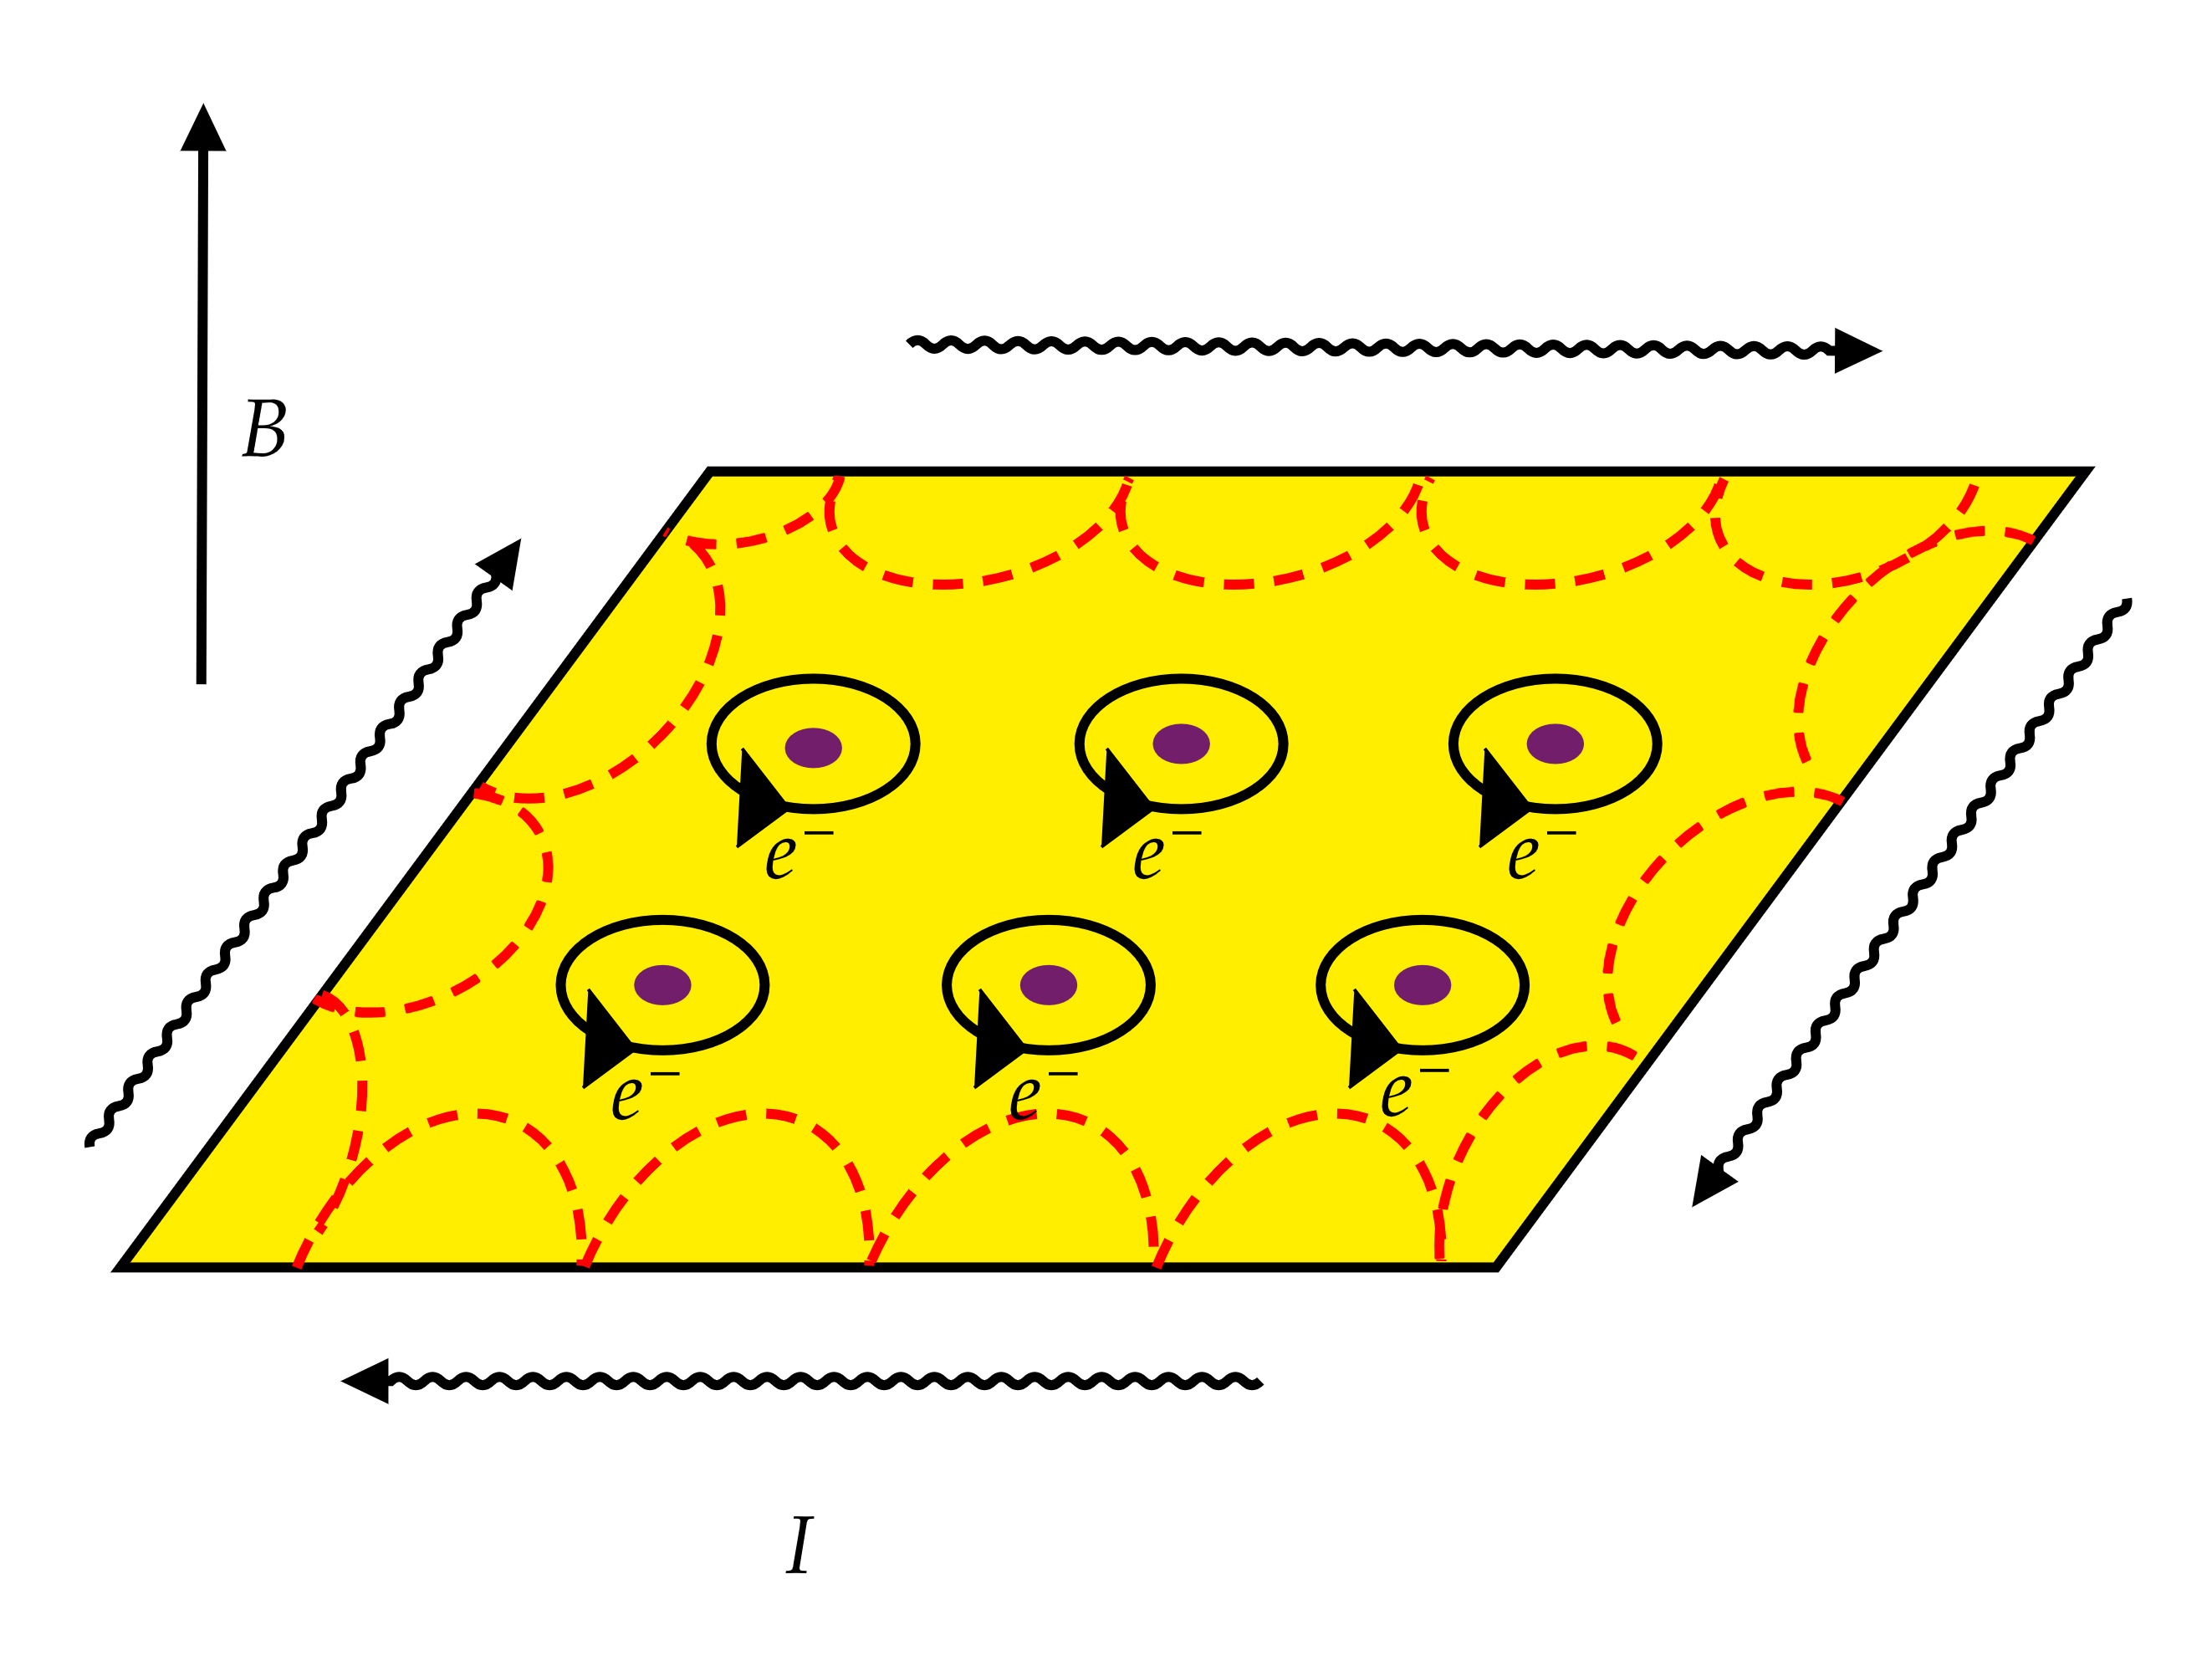
\includegraphics[width=\linewidth]{img/aillant topologic.png}
	\caption{Exemple del fenòmen de l'aïllant topològic descrit a la Secció \ref{sec:aillanttopologic}. Com es pot observar, a l'interior de la làmina, el material és aïllant ja que aquest no transporta electrons. A la frontera en canvi, sí. No és massa difícil veure que modificant la geometria de l'objecte, aquest fenòmen no s'altera. Tampoc és molt difícil veure que si a aquest objecte se li fes un forat d'un radi determinat a l'interior de la làmina, llavors l'electricitat també circularia per la frontera d'aquest. }\label{fig:aillanttopologic}
\end{figure}

\subsection{Computació amb nusos quàntics}\label{sec:nusosquantics}

La següent, és una aplicació la qual ha estat desenvolupada al llarg del darrer vicenni degut a les contribucions de Edward Witten i Alexei Kitaev en gran part. Aquesta tracta dels ordinadors quàntics, els quals prometen realitzar càlculs que es creuen impossibles per als ordinadors convencionals. Alguns d’aquests càlculs tenen una gran importància a nivel pràctic. De fet, tots els mètodes d’encriptació utilitzats per a dades altament sensibles són vulnerables a un algoritme quàntic o altre. Un exemple d'aquests és l'algorisme de Shor, un algorisme quàntic per trobar els factors primers d'un nombre enter. Mètode pel qual molts protocols de protecció de dades es veurien compromesos.\\

Aquesta secció està inspirada en els articles [\cite{computingwithquantumknots}], [\cite{braidtopologiesforquantumcomputation}] i la presentació donada per Steven Simons l'any 2021 a l'Advanced Studies Gateway Center titulada \textit{Knots, World lines and Quantum Computation} on s'estudia amb profunditat l'ús de la topologia per construïr els primers ordinadors quàntics d'una manera diferent a la convencional estudiada fins al moment, on en aquesta darrera l'importància rau en obtenir baixes temperatures -- de l'ordre de 10 milikelvins -- i camps magnètics molts forts per poder simular els efectes quàntics de la matèria.\\

El poder d’un ordinador quàntic prové del fet que opera sobre informació representada com a qubits, en lloc de bits. Un bit clàssic ordinari pot ser un 0 o un 1, i les arquitectures de microxip estàndard reforcen aquesta dicotomia de manera rigorosa. Un qubit en canvi, pot estar en un estat anomenat superposició, que comporta proporcions de 0 i 1 coexistint alhora. Es pot pensar en els possibles estats d'un qubit com els punts en una esfera. El pol nord és un 1 clàssic, el pol sud és un 0, i tots els punts intermedis són totes les superposicions possibles de 0 i 1. La llibertat que tenen els qubits per moure’s per tota l’esfera ajuda a donar als ordinadors quàntics les seves capacitats úniques.\\

Malauradament, sembla que els ordinadors quàntics són extremadament difícils de construir. Els qubits solen expressar-se com a certes propietats quàntiques de partícules atrapades, com ara ions atòmics individuals o electrons. Però els seus estats de superposició són extremadament fràgils i poden ser malmesos per les més mínimes interaccions fortuïtes amb l’entorn, que inclou tot el material que conforma l’ordinador mateix.\\

Si els qubits no estan aïllats amb cura del seu entorn, aquestes pertorbacions introduiran errors en el càlcul i en conseqüència, les propietats quàntiques del sistema es perderan. Aquest fenòmen es coneix amb el nom de decoherència quàntica i és el principal motiu que fa que els ordinadors quàntics no existeixin.\\

Per tant, la majoria dels esquemes per dissenyar un ordinador quàntic se centren en trobar maneres de minimitzar les interaccions dels qubits amb l'entorn. Els investigadors saben que si la taxa d'error es pot reduir a aproximadament un error en cada 10.000 passos, es poden implementar procediments de correcció d'errors per compensar la decoherència. Construir una màquina funcional que tingui un gran nombre de qubits aïllats prou bé per tenir una taxa d'error tan baixa és una tasca formidable que els físics estan molt lluny d'aconseguir.\\

No obtant, hi ha una manera diferent de construir un ordinador quàntic. El terme per referir-se als ordinadors que utilitzen aquesta arquitectura s'anomenen ordinadors quàntics topològics o topological quantum computer en anglès. En el seu enfocament, els delicats estats quàntics depenen del que es coneix com a propietats topològiques d'un sistema físic. Microsoft és l'empresa que tracta de crear el primer ordinador quàntic utilitzant aquesta tècnica a diferència d'altres empreses com IBM o Google que utilitzen el mètode estàndard centrant-se en les propietats quàntiques de la matèria.\\

Un ordinador quàntic topològic no opera de la mateixa manera que ho fa un ordinador convencional. Aquest realitza els seus càlculs en cordes trenades, però no cordes físiques en el sentit convencional. Més aviat, són el que els físics es refereixen com a línies del món, representacions de partícules a mesura que es mouen a través del temps i l'espai. Cal imaginar que la longitud d'una d'aquestes cordes representa el moviment d'una partícula a través del temps. Les partícules implicades són diferents dels electrons i protons que un podria imaginar primerament. Aquestes, són quasi-partícules anomenades anyons, que tenen les propietats matemàtiques desitjades\footnote{La paraula \textit{anyó} ve de l'anglès \textit{any-}, "qualsevol" en anglès. D'aquesta manera es podria pensar que aquesta partícula és "qualsevol" que no sigui una de les ja conegudes fins al moments com ara els protons, electron, neutrons, neutrins, positrons, etcètera.}. L'article [\cite{braidtopologiesforquantumcomputation}], juntament amb [\cite{topologicalquantumcomputation}] explora aquest mecanisme relacionant el càlcul del polinomi de Kauffman amb les trenes esmentades anteriorment.\\

A continuació, es dona un exemple sobre la manera com un ordinador d'aquestes característiques podria funcionar: primer, es creen parells d'anyons i es col·loquen en una línia. Cada parell d'anyons és com una partícula i la seva corresponent antipartícula, creada a partir d'energia pura. Després, es mouen parells d'anyons adjacents al voltant els uns dels altres en una seqüència acuradament determinada. La línia del món de cada anyó forma un fil, i els moviments dels anyons a mesura que s'intercanvien produeixen una trena. El càlcul quàntic ve codificat per la trena particular i es calcula mitjançant el polinomi de Kauffman de la trena. Els estats finals dels anyons, que encapsulen el resultat del càlcul, estan determinats per la trena i no per cap interacció elèctrica o magnètica. I com que la trena és topològica, deformar lleugerament els fils no canvia el resultat, de manera que està inherentment protegida de les pertorbacions externes. La idea d'utilitzar anyons per realitzar càlculs d'aquesta manera va ser proposada el 1997 per Alexei Y. Kitaev, ara a Microsoft.\\

Michael H. Freedman, actualment el director de Station Q, el centre de recerca de Microsoft dedicat a l'exploració de la computació quàntica va donar una conferència a la Universitat de Harvard a la tardor de 1988 sobre la possibilitat d'utilitzar la topologia quàntica per a la computació. Aquestes idees, publicades en un article de recerca el 1998, es basaven en el descobriment que certes quantitats matemàtiques conegudes com a invariants de nus estaven associades amb la física quàntica d'una superfície bidimensional que evoluciona en el temps. Si es pogués crear un exemple del sistema físic i realitzar una mesura adequada, l'invariant de nus seria calculat automàticament en lloc de mitjançant un càlcul llarg i inconvenient en un ordinador convencional.\\

Encara que tot això sona com teorizació salvatge molt allunyada de la realitat, experiments recents en un camp conegut com la física de l'efecte Hall quàntic fraccionari han posat l'esquema de l'anyó en una base més sòlida.